% Created by tikzDevice version 0.12.6 on 2024-03-15 15:16:54
% !TEX encoding = UTF-8 Unicode
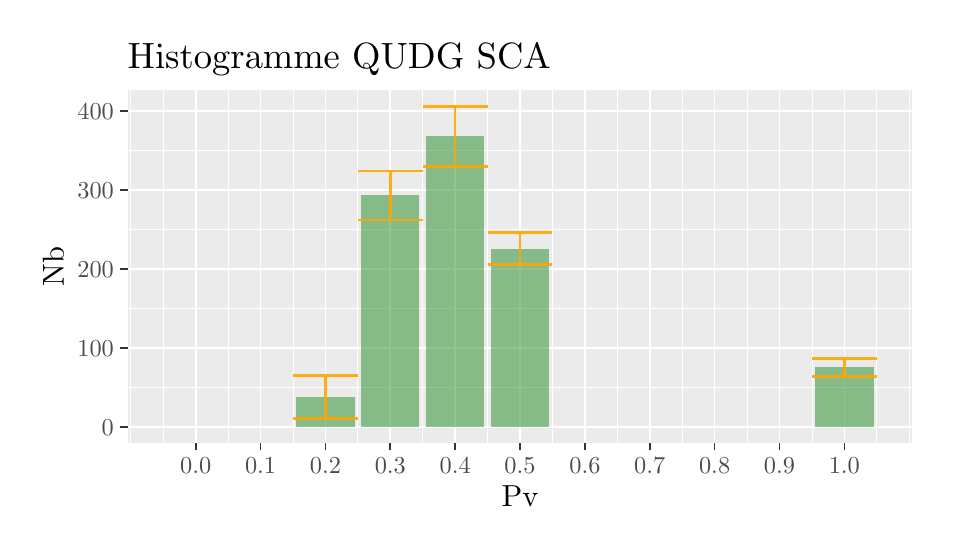
\begin{tikzpicture}[x=1pt,y=1pt]
\definecolor{fillColor}{RGB}{255,255,255}
\path[use as bounding box,fill=fillColor,fill opacity=0.00] (0,0) rectangle (325.21,180.67);
\begin{scope}
\path[clip] (  0.00,  0.00) rectangle (325.21,180.67);
\definecolor{drawColor}{RGB}{255,255,255}
\definecolor{fillColor}{RGB}{255,255,255}

\path[draw=drawColor,line width= 0.6pt,line join=round,line cap=round,fill=fillColor] (  0.00,  0.00) rectangle (325.21,180.68);
\end{scope}
\begin{scope}
\path[clip] ( 36.11, 30.69) rectangle (319.71,158.02);
\definecolor{fillColor}{gray}{0.92}

\path[fill=fillColor] ( 36.11, 30.69) rectangle (319.71,158.02);
\definecolor{drawColor}{RGB}{255,255,255}

\path[draw=drawColor,line width= 0.3pt,line join=round] ( 36.11, 50.72) --
	(319.71, 50.72);

\path[draw=drawColor,line width= 0.3pt,line join=round] ( 36.11, 79.22) --
	(319.71, 79.22);

\path[draw=drawColor,line width= 0.3pt,line join=round] ( 36.11,107.72) --
	(319.71,107.72);

\path[draw=drawColor,line width= 0.3pt,line join=round] ( 36.11,136.21) --
	(319.71,136.21);

\path[draw=drawColor,line width= 0.3pt,line join=round] ( 37.28, 30.69) --
	( 37.28,158.02);

\path[draw=drawColor,line width= 0.3pt,line join=round] ( 49.00, 30.69) --
	( 49.00,158.02);

\path[draw=drawColor,line width= 0.3pt,line join=round] ( 72.44, 30.69) --
	( 72.44,158.02);

\path[draw=drawColor,line width= 0.3pt,line join=round] ( 95.88, 30.69) --
	( 95.88,158.02);

\path[draw=drawColor,line width= 0.3pt,line join=round] (119.32, 30.69) --
	(119.32,158.02);

\path[draw=drawColor,line width= 0.3pt,line join=round] (142.76, 30.69) --
	(142.76,158.02);

\path[draw=drawColor,line width= 0.3pt,line join=round] (166.19, 30.69) --
	(166.19,158.02);

\path[draw=drawColor,line width= 0.3pt,line join=round] (189.63, 30.69) --
	(189.63,158.02);

\path[draw=drawColor,line width= 0.3pt,line join=round] (213.07, 30.69) --
	(213.07,158.02);

\path[draw=drawColor,line width= 0.3pt,line join=round] (236.51, 30.69) --
	(236.51,158.02);

\path[draw=drawColor,line width= 0.3pt,line join=round] (259.95, 30.69) --
	(259.95,158.02);

\path[draw=drawColor,line width= 0.3pt,line join=round] (283.39, 30.69) --
	(283.39,158.02);

\path[draw=drawColor,line width= 0.3pt,line join=round] (306.82, 30.69) --
	(306.82,158.02);

\path[draw=drawColor,line width= 0.3pt,line join=round] (318.54, 30.69) --
	(318.54,158.02);

\path[draw=drawColor,line width= 0.6pt,line join=round] ( 36.11, 36.47) --
	(319.71, 36.47);

\path[draw=drawColor,line width= 0.6pt,line join=round] ( 36.11, 64.97) --
	(319.71, 64.97);

\path[draw=drawColor,line width= 0.6pt,line join=round] ( 36.11, 93.47) --
	(319.71, 93.47);

\path[draw=drawColor,line width= 0.6pt,line join=round] ( 36.11,121.96) --
	(319.71,121.96);

\path[draw=drawColor,line width= 0.6pt,line join=round] ( 36.11,150.46) --
	(319.71,150.46);

\path[draw=drawColor,line width= 0.6pt,line join=round] ( 60.72, 30.69) --
	( 60.72,158.02);

\path[draw=drawColor,line width= 0.6pt,line join=round] ( 84.16, 30.69) --
	( 84.16,158.02);

\path[draw=drawColor,line width= 0.6pt,line join=round] (107.60, 30.69) --
	(107.60,158.02);

\path[draw=drawColor,line width= 0.6pt,line join=round] (131.04, 30.69) --
	(131.04,158.02);

\path[draw=drawColor,line width= 0.6pt,line join=round] (154.47, 30.69) --
	(154.47,158.02);

\path[draw=drawColor,line width= 0.6pt,line join=round] (177.91, 30.69) --
	(177.91,158.02);

\path[draw=drawColor,line width= 0.6pt,line join=round] (201.35, 30.69) --
	(201.35,158.02);

\path[draw=drawColor,line width= 0.6pt,line join=round] (224.79, 30.69) --
	(224.79,158.02);

\path[draw=drawColor,line width= 0.6pt,line join=round] (248.23, 30.69) --
	(248.23,158.02);

\path[draw=drawColor,line width= 0.6pt,line join=round] (271.67, 30.69) --
	(271.67,158.02);

\path[draw=drawColor,line width= 0.6pt,line join=round] (295.10, 30.69) --
	(295.10,158.02);
\definecolor{fillColor}{RGB}{34,139,34}

\path[fill=fillColor,fill opacity=0.50] ( 97.05, 36.47) rectangle (118.15, 47.21);

\path[fill=fillColor,fill opacity=0.50] (120.49, 36.47) rectangle (141.58,120.04);

\path[fill=fillColor,fill opacity=0.50] (143.93, 36.47) rectangle (165.02,141.38);

\path[fill=fillColor,fill opacity=0.50] (167.37, 36.47) rectangle (188.46,100.83);

\path[fill=fillColor,fill opacity=0.50] (284.56, 36.47) rectangle (305.65, 57.88);
\definecolor{drawColor}{RGB}{255,165,0}

\path[draw=drawColor,draw opacity=0.90,line width= 0.9pt,line join=round] ( 95.88, 54.93) --
	(119.32, 54.93);

\path[draw=drawColor,draw opacity=0.90,line width= 0.9pt,line join=round] (107.60, 54.93) --
	(107.60, 39.49);

\path[draw=drawColor,draw opacity=0.90,line width= 0.9pt,line join=round] ( 95.88, 39.49) --
	(119.32, 39.49);

\path[draw=drawColor,draw opacity=0.90,line width= 0.9pt,line join=round] (119.32,128.93) --
	(142.76,128.93);

\path[draw=drawColor,draw opacity=0.90,line width= 0.9pt,line join=round] (131.04,128.93) --
	(131.04,111.16);

\path[draw=drawColor,draw opacity=0.90,line width= 0.9pt,line join=round] (119.32,111.16) --
	(142.76,111.16);

\path[draw=drawColor,draw opacity=0.90,line width= 0.9pt,line join=round] (142.76,152.23) --
	(166.19,152.23);

\path[draw=drawColor,draw opacity=0.90,line width= 0.9pt,line join=round] (154.47,152.23) --
	(154.47,130.52);

\path[draw=drawColor,draw opacity=0.90,line width= 0.9pt,line join=round] (142.76,130.52) --
	(166.19,130.52);

\path[draw=drawColor,draw opacity=0.90,line width= 0.9pt,line join=round] (166.19,106.64) --
	(189.63,106.64);

\path[draw=drawColor,draw opacity=0.90,line width= 0.9pt,line join=round] (177.91,106.64) --
	(177.91, 95.02);

\path[draw=drawColor,draw opacity=0.90,line width= 0.9pt,line join=round] (166.19, 95.02) --
	(189.63, 95.02);

\path[draw=drawColor,draw opacity=0.90,line width= 0.9pt,line join=round] (283.39, 61.18) --
	(306.82, 61.18);

\path[draw=drawColor,draw opacity=0.90,line width= 0.9pt,line join=round] (295.10, 61.18) --
	(295.10, 54.58);

\path[draw=drawColor,draw opacity=0.90,line width= 0.9pt,line join=round] (283.39, 54.58) --
	(306.82, 54.58);
\end{scope}
\begin{scope}
\path[clip] (  0.00,  0.00) rectangle (325.21,180.67);
\definecolor{drawColor}{gray}{0.30}

\node[text=drawColor,anchor=base east,inner sep=0pt, outer sep=0pt, scale=  0.88] at ( 31.16, 33.44) {0};

\node[text=drawColor,anchor=base east,inner sep=0pt, outer sep=0pt, scale=  0.88] at ( 31.16, 61.94) {100};

\node[text=drawColor,anchor=base east,inner sep=0pt, outer sep=0pt, scale=  0.88] at ( 31.16, 90.44) {200};

\node[text=drawColor,anchor=base east,inner sep=0pt, outer sep=0pt, scale=  0.88] at ( 31.16,118.93) {300};

\node[text=drawColor,anchor=base east,inner sep=0pt, outer sep=0pt, scale=  0.88] at ( 31.16,147.43) {400};
\end{scope}
\begin{scope}
\path[clip] (  0.00,  0.00) rectangle (325.21,180.67);
\definecolor{drawColor}{gray}{0.20}

\path[draw=drawColor,line width= 0.6pt,line join=round] ( 33.36, 36.47) --
	( 36.11, 36.47);

\path[draw=drawColor,line width= 0.6pt,line join=round] ( 33.36, 64.97) --
	( 36.11, 64.97);

\path[draw=drawColor,line width= 0.6pt,line join=round] ( 33.36, 93.47) --
	( 36.11, 93.47);

\path[draw=drawColor,line width= 0.6pt,line join=round] ( 33.36,121.96) --
	( 36.11,121.96);

\path[draw=drawColor,line width= 0.6pt,line join=round] ( 33.36,150.46) --
	( 36.11,150.46);
\end{scope}
\begin{scope}
\path[clip] (  0.00,  0.00) rectangle (325.21,180.67);
\definecolor{drawColor}{gray}{0.20}

\path[draw=drawColor,line width= 0.6pt,line join=round] ( 60.72, 27.94) --
	( 60.72, 30.69);

\path[draw=drawColor,line width= 0.6pt,line join=round] ( 84.16, 27.94) --
	( 84.16, 30.69);

\path[draw=drawColor,line width= 0.6pt,line join=round] (107.60, 27.94) --
	(107.60, 30.69);

\path[draw=drawColor,line width= 0.6pt,line join=round] (131.04, 27.94) --
	(131.04, 30.69);

\path[draw=drawColor,line width= 0.6pt,line join=round] (154.47, 27.94) --
	(154.47, 30.69);

\path[draw=drawColor,line width= 0.6pt,line join=round] (177.91, 27.94) --
	(177.91, 30.69);

\path[draw=drawColor,line width= 0.6pt,line join=round] (201.35, 27.94) --
	(201.35, 30.69);

\path[draw=drawColor,line width= 0.6pt,line join=round] (224.79, 27.94) --
	(224.79, 30.69);

\path[draw=drawColor,line width= 0.6pt,line join=round] (248.23, 27.94) --
	(248.23, 30.69);

\path[draw=drawColor,line width= 0.6pt,line join=round] (271.67, 27.94) --
	(271.67, 30.69);

\path[draw=drawColor,line width= 0.6pt,line join=round] (295.10, 27.94) --
	(295.10, 30.69);
\end{scope}
\begin{scope}
\path[clip] (  0.00,  0.00) rectangle (325.21,180.67);
\definecolor{drawColor}{gray}{0.30}

\node[text=drawColor,anchor=base,inner sep=0pt, outer sep=0pt, scale=  0.88] at ( 60.72, 19.68) {0.0};

\node[text=drawColor,anchor=base,inner sep=0pt, outer sep=0pt, scale=  0.88] at ( 84.16, 19.68) {0.1};

\node[text=drawColor,anchor=base,inner sep=0pt, outer sep=0pt, scale=  0.88] at (107.60, 19.68) {0.2};

\node[text=drawColor,anchor=base,inner sep=0pt, outer sep=0pt, scale=  0.88] at (131.04, 19.68) {0.3};

\node[text=drawColor,anchor=base,inner sep=0pt, outer sep=0pt, scale=  0.88] at (154.47, 19.68) {0.4};

\node[text=drawColor,anchor=base,inner sep=0pt, outer sep=0pt, scale=  0.88] at (177.91, 19.68) {0.5};

\node[text=drawColor,anchor=base,inner sep=0pt, outer sep=0pt, scale=  0.88] at (201.35, 19.68) {0.6};

\node[text=drawColor,anchor=base,inner sep=0pt, outer sep=0pt, scale=  0.88] at (224.79, 19.68) {0.7};

\node[text=drawColor,anchor=base,inner sep=0pt, outer sep=0pt, scale=  0.88] at (248.23, 19.68) {0.8};

\node[text=drawColor,anchor=base,inner sep=0pt, outer sep=0pt, scale=  0.88] at (271.67, 19.68) {0.9};

\node[text=drawColor,anchor=base,inner sep=0pt, outer sep=0pt, scale=  0.88] at (295.10, 19.68) {1.0};
\end{scope}
\begin{scope}
\path[clip] (  0.00,  0.00) rectangle (325.21,180.67);
\definecolor{drawColor}{RGB}{0,0,0}

\node[text=drawColor,anchor=base,inner sep=0pt, outer sep=0pt, scale=  1.10] at (177.91,  7.64) {Pv};
\end{scope}
\begin{scope}
\path[clip] (  0.00,  0.00) rectangle (325.21,180.67);
\definecolor{drawColor}{RGB}{0,0,0}

\node[text=drawColor,rotate= 90.00,anchor=base,inner sep=0pt, outer sep=0pt, scale=  1.10] at ( 13.08, 94.35) {Nb};
\end{scope}
\begin{scope}
\path[clip] (  0.00,  0.00) rectangle (325.21,180.67);
\definecolor{drawColor}{RGB}{0,0,0}

\node[text=drawColor,anchor=base west,inner sep=0pt, outer sep=0pt, scale=  1.32] at ( 36.11,166.08) {Histogramme QUDG SCA};
\end{scope}
\end{tikzpicture}
